\chapter{Implementierung}
\label{cha:implementierung}

Dieses Kapitel bietet einen Überblick über die Implementierung der Bibliothek. Dabei werden einige Stellen aus dem Quellcode vorgestellt und ihre Funktionalität näher beschrieben. Dieses Kapitel enthält ebenfalls Durchführung und Beschreibung entwickelten Testfälle.

\section{Strukturierung und Typisierung in Python}
\label{sec:impl_structure_problems}

% - Module aufgeteilt in mehrere Dateien -> Was exportiert wird in __init__.py des Ordners definiert
Zu Beginn der Implementierung wurde die grundlegende Struktur des Codes festgelegt. Die Code-Basis der Bibliothek ist auf zwei Python-Module aufgeteilt: \emph{scikit\_charts} und \emph{tests}. \emph{scikit\_charts} beinhaltet den gesamten Code der Bibliothek und besitzt drei darunterliegende Module. \emph{metrics} für die Metrikberechnung, \emph{charts} für die Implementierungen der Diagramme und \emph{shared} für geteilten Code zwischen den Diagrammen. \emph{tests} beinhaltet alle Unit- und Integrationtests des Projektes. Um die Abhängigkeiten sowie die Erstellung der finalen Pakete zu Verwalten wird \emph{poetry}\footnote{https://python-poetry.org/} verwendet. Dieses Werkzeug erlaubt es, das gesamte Projekt über eine einzelne \emph{pyproject.toml} Datei zu definieren. In diesem werden die minimalen Versionen der Abhängigkeiten definiert. Sie beinhaltet auch die Metadaten der Bibliothek. In den Modulen sind die Implementierungen auf einzelne Dateien aufgeteilt. Diese beinhalten sowohl Klassen, Funktionen als auch Definitionen von Typen und Konstanten. In der Wurzel jedes Moduls liegt eine \emph{\_\_init\_\_.py} Datei. In dieser wird definiert, welche Inhalte der einzelnen Dateien von außerhalb des Moduls sichtbar sind.\\\\
% - Herausforderung: Typisierung von Python sowie fehlende Typen by Pycharm
\noindent Eine allgemeine Herausforderung, welche sich während der Implementierung stellte, war das Typ-System von Python. Durch die dynamische Typisierung können Variablen zur Laufzeit jeden beliebigen Datentyp annehmen. Aus diesem Grund gibt es in Python die Möglichkeit Typ-Informationen zu hinterlegen\footnote{https://docs.python.org/3/library/typing.html}. Diese werden sowohl vom statische Code-Analyse-Tools als auch von Pycharm zur Unterstützung der Entwickler:innen verwendet. Manche Bibliotheken wie Matplot haben jedoch keine Typinformationen hinterlegt. Dadurch ist es notwendig oft die Dokumentation oder sogar den originalen Sourcecode nach dem Typ zu überprüfen. Dadurch wird der Einstieg vor allem für Erstanwender:innen einer Bibliothek erschwert. Um diesen Fall für Anwender:innen von Scikit-charts zu vermeiden, wurde während der Entwicklung jede Variable mit Typinformationen hinterlegt.

%   - Python module -> Richtig konfigurieren; Tests probleme beim erkennen??


\section{Implementierung der Metriken}
\label{sec:impl_metrics}

% ToDo: Einfügen von Code-Stücken?

% - Index wird implizit von DataFrame verwaltet
Bei den Metriken wurden einige Verbesserungen gegenüber der Planung umgesetzt. Der Index wird nicht mehr als eigene Spalte gespeichert. Dieser wird bereits automatisch von Pandas verwaltet.
% - Enum für Zugriff auf Metrik-Spalten -> Keine Magic-Strings + Helfer für Zugriff auf feature columns
Um den Zugriff auf die Metriken des Dataframe zu verbessern, wurde das Enum \emph{MetricEnum} eingeführt. In dieser sind alle Spaltennamen der Metriken als Werte hinterlegt. Die einzelnen Einträge des Enums können dadurch für den Zugriff auf die jeweiligen Spalten verwendet werden. Dadurch gibt es keine Abhängigkeit mehr auf Magicstrings, welche eine mögliche Fehlerquelle darstellen. Die zusätzliche Hilfsfunktion \emph{get\_feature\_columns} der Enum-Klasse erleichtert außerdem die Arbeit mit den Spalten für die Einflusswerte. Die Funktion gibt die Namen dieser dynamisch generierten\linebreak Spalten aus einem DataFrame als Liste zurück.\\\\
% - Metrik-Berechnung -> Fehler in predict -> Throw exception. Warum? Debug von Predict-Funktion + Konsistente Daten erfordert, da keine andere Daten wie z.B. NaN eingefügt werden. Muss später nicht gehandelt werden.
% - Interne Datentypen -> float64 -> Definition für fixen Typ
\noindent Eine weitere mögliche Fehlerquelle stellen der Datentyp der gespeicherten Metriken, sowie die übergebene predict-Funktion dar. Der interne Datentyp zur Speicherung wurde daher auf \emph{float64} festgelegt. Dadurch kann sichergestellt werden, dass alle übergebenen Daten konsistent gespeichert werden. Für die predict-Funktion wurde eine eigene \emph{PredictionException} definiert. Dieser wird geworfen, wenn ein Fehler während der\linebreak Vorhersage eines Wertes auftritt. Dadurch kann sichergestellt werden, dass die Metriken nie in einem inkonsistenten Zustand zurückgegeben werden. Eine Alternative wäre das Einfügen von NaN-Werten\footnote{Not a Number} gewesen. Auf diese müsste während der Visualisierung jedoch explizit geprüft werden. Dies würde einen zusätzlichen Aufwand darstellen.

\section{Implementierung von Linien- und Streudiagramm}
\label{sec:impl_line_scatter}

Wie in dem Design (Abschnitt \ref{sec:design_aufbau_diagramme}) beschrieben, sind alle Diagramme mittels einer Funktion und Klasse implementiert. Bei Linien- und Streudiagramm werden innerhalb dieser Funktion die Metriken gesammelt. Mithilfe dieser erfolgt dann die Instanzierung der Klassen. Um das Figure-Objekt für die Rückgabe zu erhalten ist in allen Diagrammklassen eine \emph{get\_figure} Funktion enthalten.\\

\begin{figure}[H]
    \centering
    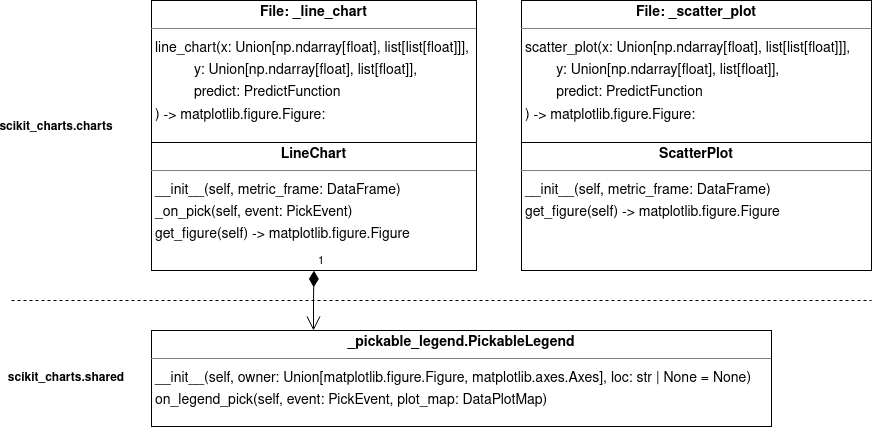
\includegraphics[width=\textwidth]{images/uml_scatter_line_chart.png}
    \caption{Klassendiagramm von Linien- und Streudiagramm}
    \label{fig:uml_line_scatter}
\end{figure}

\subsection{Erstellung des Streudiagramms}
\label{subsec:impl_scatter}
%   - Keine Implementierung von Zoom / Bewegen des Diagramms -> Wird bereits automatisch in interaktiven Umgebungen von Matlab unterstützt
% - wie konfiguriert man interaktivität in Matplotlib
\noindent Die Implementierung des Streudiagramms konnte rein durch die von Matplot zur Verfügung gestellten Funktionen erfolgen. Das grundlegende Diagramm kann mittels eines einzelnen Funktionsaufruf erstellt werden. Sowohl die 45°-Linie als auch das Gitter im Hintergrund können direkt über das Axes-Objekt konfiguriert werden. Der Zoom, sowie die Bewegung des angezeigten Bereiches im Diagramm werden von Matplot out-of-the-box zur Verfügung gestellt. Dafür muss das Diagramm mit einem interaktiven Backend von Matplot gestartet werden.

\subsection{Backends in Matplot}
\label{subsec:impl_backend}
%   - Weitere Abhängigkeit ipympl um dynamische Interaktion in Jupyter zu unterstützen -> Aktivieren mittels %matplotlib widget
\noindent Bei den Backends\footnote{https://matplotlib.org/stable/users/explain/backends.html} von Matplot handelt es sich um Implementierungen der Darstellung für verschiedene grafische Ausgaben. Diese sind entweder statisch für Dateien (PNG, SVG, ...) oder interaktiv basierend auf verschiedenen GUI-Plattformen. In den meisten Fällen wählt die Bibliothek automatisch das passende interaktive Backend für die aktuelle Plattform. Die IDE Pycharm, sowie Jupyter Notebook benötigen jedoch weitere Konfigurationen. In Pycharm muss das passende Backend der aktuellen Plattform mithilfe von `matplotlib.use(...)` konfiguriert werden. Ansonsten wird standardmäßig ein nicht interaktives Backend ausgewählt. Um die Interaktivität in Jupyter Notebook zu ermöglichen wurde eine neue Abhängigkeit auf \emph{ipympl} zum Projekt hinzugefügt. Dabei handelt es sich um ein Matplot Backend für Jupyter Notebook. Anwender:innen können dieses Backend in Jupyter Notebook durch das Einfügen der Zeile \emph{\%matplotlib widget} aktivieren. 

\subsection{Liniendiagramm und Hilfsklassen}
\label{subsec:impl_linien_helper}
\noindent Liniendiagramme werden in Matplot explizit unterstützt. Dafür kann die \emph{plot}-Funktion verwendet werden. Für die interaktive Legende wird jedoch eine Hilfsklasse benötigt. Daher wurde eine Klasse \emph{PickableLegend} erstellt. Diese kümmert sich um das dynamische Ausblenden von Linien durch das Klicken auf den jeweiligen Eintrag in der Legende. Unterstützt wird dabei jedes Figure- oder Axes-Objekt, auf welchem bereits Daten dargestellt wurden. Während der Instantiierung der PickableLegend wird für diese Figure/Axes eine neue Legende erstellt. Diese ist konfiguriert um \emph{on\_pick} Events für Matplot zu generieren. In der Liniendiagrammklasse wird auf diese Events\linebreak reagiert. Wenn ein on\_pick-Event erkannt wird, erfolgt ein Aufruf von \emph{legend\_pic} in der PickableLegend. Diese kümmert sich um das ausblenden der Daten basierend auf dem gewählten Element. Die mitgegebene Map gibt dabei an, welche dargestellten Daten zu welchem Legendeneintrag passen.

\subsection{Matplot Interaktivität und der Garbage-Collector}
\label{subsec:impl_interact_problems}
%   - Click-Events -> Schwer zu koppeln da aktivert werden muss -> Schwer richtige Referenzen zu bekommen + Koppeln mit anderen Daten eine herausforderung
%   - Herausforderung von Referenzen -> Müssen gehalten werden damit interaktivität (Widgets) funtkioniert -> Implementierungen müssen deshalb als Klassen erstellt werden
\noindent Eine Herausforderung während der Implementierung stellte der Lebenszyklus von Python-Objekten dar. Referenzen auf Callback, dargestellte Daten sowie Legende müssen während der gesamten Lebensdauer der Darstellung gespeichert werden. Passiert dies nicht, kann es sein, dass die Objekte vom Garbage Collector entfernt werden. In diesem Fall geht die Interaktivität verloren. Aus diesem Grund sind alle dynamischen UI-Elemente als Klassen implementiert.

\pagebreak

\section{Implementierung des Blasendiagramms}
\label{sec:impl_bubble}

Der Fokus beim Blasendiagramm lag auf dessen hoher Konfigurierbarkeit. Aus diesem Grund einstanden während dessen Entwicklung die meisten Hilfsklassen und Funktionen. Dies ist auch in dem UML-Diagramm des Diagramms in Abbildung \ref{fig:uml_bubble} ersichtlich.

\begin{figure}[H]
    \centering
    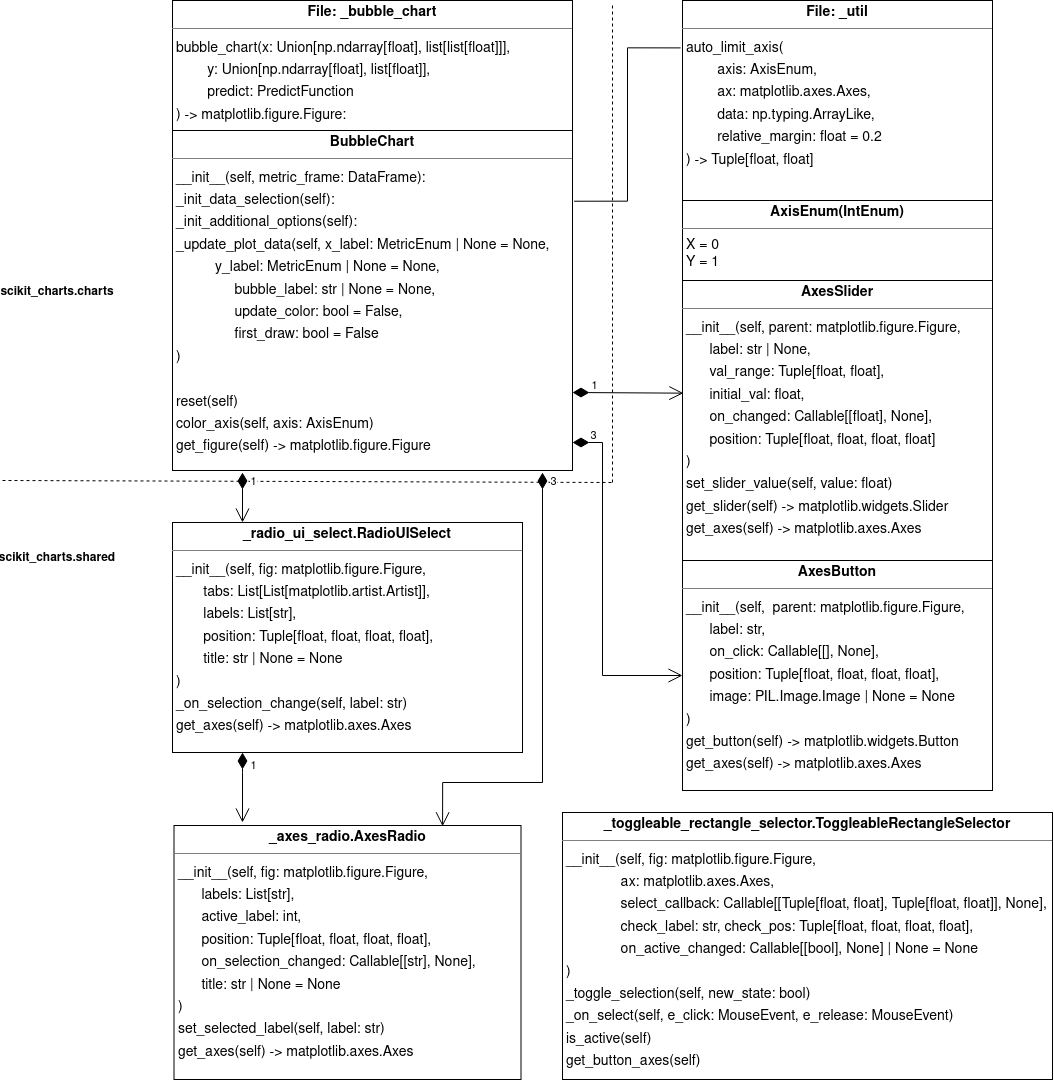
\includegraphics[width=\textwidth]{images/uml_bubble_chart.png}
    \caption{Klassendiagramm des Blasendiagramms}
    \label{fig:uml_bubble}
\end{figure}

\subsection{Hilfsklassen des Blasendiagramms}
\label{subsec:impl_linien_helper}
% - Selektierung von Werten für Achsen
% - Mehrere zusätzliche UI-Elemente (RadioSelect, Axes impls)
Während der Implementierung des Blasendiagramms stellten sich gleich mehrere\linebreak Herausforderungen auf einmal. Die Erste war die Auswahl der Metriken für Achsen und Blasengröße. Da Matplot kein Drop-Down-Menü zur Verfügung stellt, erfolgt die Auswahl über Radio-Buttons. Diese werden in einer Seitenleiste neben dem Diagramm angezeigt. Für die Radio-Buttons wurde eine eigene Hilfsklasse namens \emph{AxesRadio} erstellt. Solche Hilfsklassen, mit dem Namensschema \emph{Axes<UI-Element>} existieren in der Bibliothek für verschiedene UI-Elemente. Beispielsweise auch für Buttons und Slider. Es handelt sich dabei bei allen um einfache Wrapper um die jeweilige Klasse aus Matplot. Diese Hilfsklassen kümmern sich intern um die Positionierung und Konfiguration der Matplot Objekte, sowie das Halten der notwendigen Referenzen. Dadurch wird die Komplexität und Größe der eigentlichen Diagrammklassen verringert. Sie können außerdem von Anwender:innen in eigenen Implementierungen wiederverwendet werden.

\subsection{Aktualisierung der Daten im Diagramm}
\label{subsec:impl_bubble_data_update}
% - Gebündelte Update-Funktion -> Setzen von Daten + Update des Plots
%   - Aufruf von self._plot_data.remove() für effizienteres löschen als figure.clear
\noindent Die Auswahl eines Wertes in der Seitenleiste führt intern zu einem Update der angezeigten Daten. Dafür wird die \emph{\_update\_plot\_data(...)} Funktion aufgerufen. Diese kümmert sich sowohl um das setzen der internen Attribute als auch um das neue Zeichnen der Daten. Als Argumente wird übergeben, ob und welche Daten sich geändert haben. Gleichbleibende Werte werden nicht aktualisiert. Dadurch werden nur die notwendigen Teile im Diagramm neu aufgezeichnet. Durch das Bündeln in einer einzelnen Funktion bleibt der Aufruf zum Neuzeichnen der Daten konsistent. Um das Zeichnen weiter zu optimieren, werden die gezeichneten Daten zwischengespeichert. Sind diese Daten beim nächsten Aufruf verfügbar, werden sie von dem Figure-Objekt entfernt, anstatt die gesamte Figure zurückzusetzen.

\subsection{Layouting des Blasendiagramms}
\label{subsec:impl_bubble_layout}
% - Layouting der UI-Elemente und Bereiche + Warum so implementiert
%   - Herausforderung: Layouting für buttons + keine DropDownMenüs per default -> Plotly wäre einfacher gewesen
\noindent Eine weitere Herausforderung bei der Entwicklung war das Layout des Diagramms. Die hohe Anzahl an Metriken bedeutet, dass viele Einträge gleichzeitig angezeigt werden müssen. Dementsprechend benötigt die Metrikauswahl viel Platz. Wie in HeuristicLab würde ein Drop-Down-Menü dafür Abhilfe schaffen. Als Alternative dazu, wurde neue Radio-Buttons hinzugefügt, mithilfe welcher die angezeigten Einstellungen gewechselt werden können. Dabei kann zwischen X- sowie Y-Achse, Blasengröße und weiteren Optionen\linebreak gewählt werden. Das ganze wurde in einer Hilfsklasse namens \emph{RadioUISelect} implementiert. Dieses Element versteckt automatisch alle UI-Elemente, welche nicht zum aktuell gewählten Eintrag gehören. Dadurch können die vielen Optionen mit relativ geringen Platzverbrauch angeboten werden.

\subsection{Mausinteraktionen und Datenselektierung}
\label{subsec:impl_mouse}

\noindent Das Blasendiagramm in HeuristicLab unterstützt die Selektion und Manipulation einzelner Blasen mithilfe der Maus. Die Implementierung dieser Funktion war ebenfalls für Scikit-charts angedacht. Die Implementierung musste jedoch aus zeitlichen Gründen abgebrochen werden. Das Problem war die Färbung sowie Ausblendung einzelner Datenpunkte. Die bestehende Implementierung führte dabei zu Problem beim Wechseln der angezeigten Metriken. Die Bereichsauswahl selbst, wird explizit von Matplot unterstützt. Dafür werden sogenannte Selektoren bereitgestellt. Diese können zu einem Figure- oder Axes-Objekt hinzugefügt werden. Über einen Callback kann am Ende einer Auswahl auf den gewählten Bereich reagiert werden. Da die Bereichsauswahl nicht dauerhaft aktiv sein soll, ist es notwendig diese umzuschalten. Dafür wurde eine Hilfsklasse namens \emph{ToggleableRectangleSelector} implementiert. Diese fügt zusätzlich zu einem Selektor eine Checkbox in das Diagramm ein. Beim umschalten dieser Checkbox wird ebenfalls die Bereichsauswahl umgeschaltet und der zuletzt gewählte Bereich ausgeblendet. Um auf die Auswahl reagieren zu können, werden zwei Callbacks übergeben. Der eine erhält die minimale und maximale Position des Bereiches, sobald sich dieser ändert. Der Bereich kann dadurch in der Diagrammklasse abgespeichert werden. Der andere Callback reagiert auf das Umschalten des Selectors. Dadurch können gespeicherte Werte in der Klasse wieder invalidiert werden.


\section{Implementierung des Schnittdiagramms}
\label{sec:impl_partial_dependency}

Beim Schnittdiagramm handelte es sich um die wohl komplexeste Diagrammimplementierung. Die Herausforderungen lagen dabei bei der Berechnung und Verwaltung der Daten, sowie der komplexen Interaktivität. Das Diagramm wurde deshalb in zwei\linebreak Klassen unterteilt. Zusätzlich wurde eine weitere Hilfsklasse dafür entwickelt.

\begin{figure}[H]
    \centering
    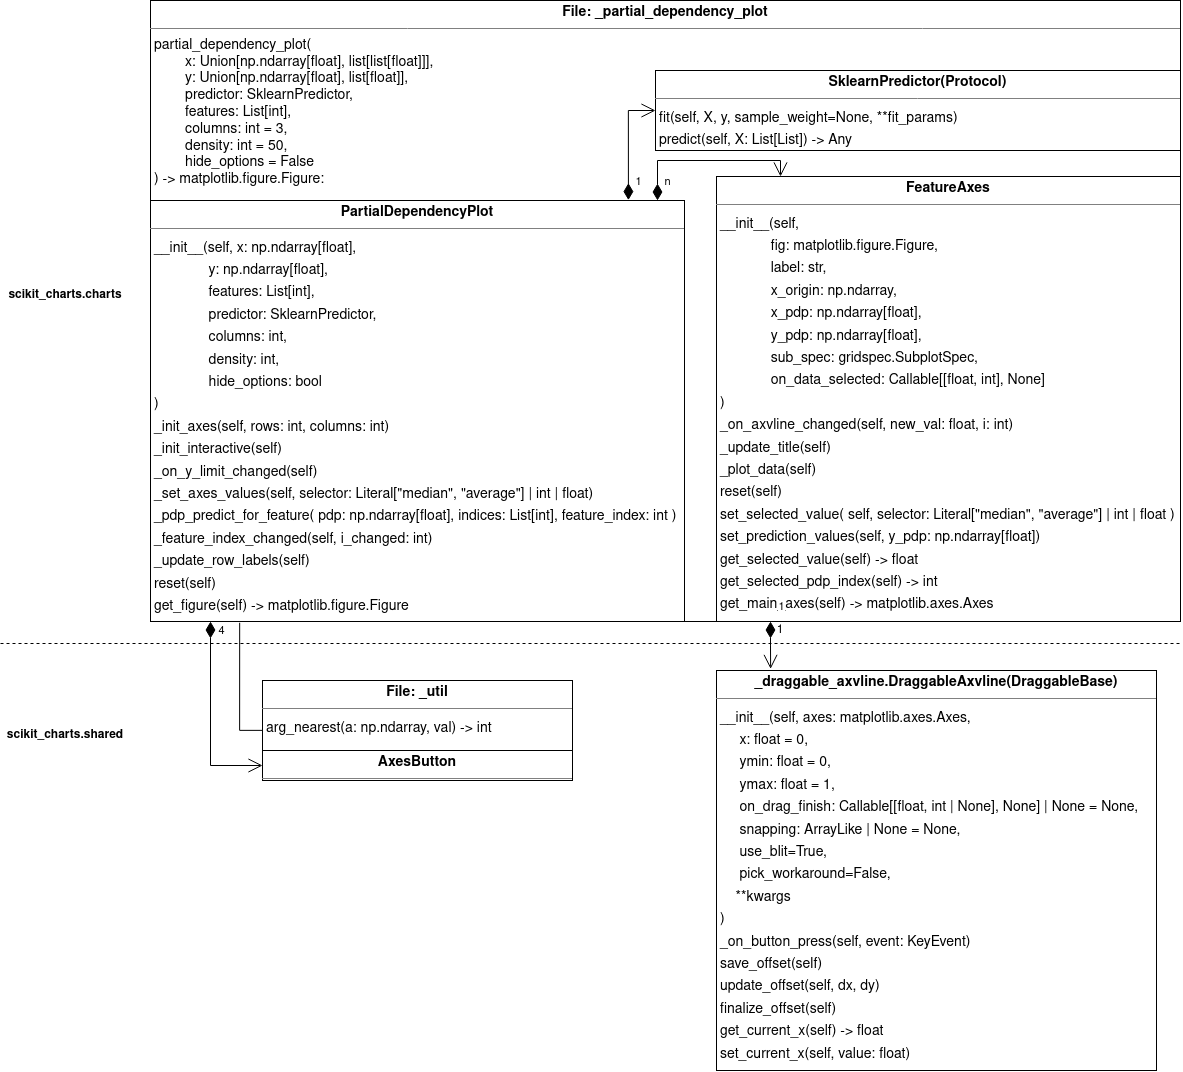
\includegraphics[width=0.95\textwidth]{images/uml_partial_dependence.png}
    \caption{Klassendiagramm des Schnittdiagramms}
    \label{fig:uml_partial_dependence}
\end{figure}

\subsection{Berechnung der Abhängigkeiten}
\label{subsec:pdp_calculation_visualization}
% - SklearnPredictor
Zur Berechnung der \emph{partial dependence} (Abschnitt \ref{sec:partial_dependence}) wird die Funktion\linebreak \emph{sklearn.inspection.partial\_dependence(..)} verwendet. Dafür wird ein in Scikit-learn trainiertes Modell benötigt. Da Scikit-learn dafür keine Typinformationen bereitstellt, wird eine eigene \emph{Protocol}-Klasse implementiert. Ein \emph{Protocol}\footnote{https://peps.python.org/pep-0544/} in Python beschreibt den Typ eines Objektes basierend auf dessen Struktur. Das Schnittdiagramm benötigt daher einen \emph{SklearnPredictor}. Diese Protocolklasse definiert ein Objekt welches eine \emph{fit} und \emph{predict} Funktion besitzt. Diese werden mindestens für die partial\_dependence-Funktion benötigt.\\\\
% - Scikitlearn für Berechnung von Partial-Dependence
% Index von Feature-Wert zum Zugriff auf Predict-Liste
% Reihenfolge für Zugriff die gleiche wie originale Indicies
% Feature-Werte + Werte aus Predict-Liste werden in Kacheln angezeigt
\noindent Das Ergebnis der partial\_dependence-Funktion ist eine Map ähnliche Datenstruktur für eine angegebene Liste an Einflussvariablen. Ein Eintrag im Ergebnis beinhaltet mögliche Werte für alle gewählten Einflussvariablen. Ein weiterer Eintrag ist eine $m^n$ tief geschachtelte Liste, welche die Vorhersagen für die Wert-Kombinationen\linebreak beinhaltet. Variable $n$ beschreibt dabei die Anzahl der gewählten Einflussvariablen. Variable $m$ beschreibt die Anzahl an generierten Werten pro Einflussvariable. Der Zugriff auf das Vorhersagen-Array ($pd$) erfolgt über die Indices der gewählten Variablenwerte: $pd[n_0][n_{...}][n_n]$. Um dementsprechend in einer Wertkombination alle Vorhersagen für\linebreak eine Variable zu erhalten, müssen an der Position dieser Variable alle möglichen Indices gewählt werden. Da dieser Zugriff durch die Komplexität Fehleranfällig ist, wurde er in die Funktion \emph{\_pdp\_predict\_for\_feature(..)} ausgelagert. Diese gibt die Vorhersage für eine Einflussvariable basierend auf den Wert-Indices zurück. Ein Beispiel für den Zugriff in Python ist in der nachfolgenden Tabelle ersichtlich.\\

\begin{table}[H]
\centering
    \begin{tabular}{lll}
        \textbf{Einflussvariable} & \textbf{x1} & \textbf{x2} \\ [0.4cm]
        \textbf{Generierte Werte} & {[}1; 2.5; 3{]} & {[}0; 3; 4{]} \\ [0.4cm]
        \textbf{Generierte Vorhersage (pd)} & \multicolumn{2}{l}{{[}{[}1; 4; 5{]}, {[}2,5; 5,5; 6,5{]}, {[}3; 6; 7{]}{]}} \\ [0.4cm]
        \textbf{Gewählte Variablenwerte} & 2,5 & 4 \\ [0.4cm]
        \textbf{\begin{tabular}[c]{@{}l@{}}Vorhersage basierend auf\\ Wert anderer Variable\end{tabular}} & \begin{tabular}[c]{@{}l@{}}pd{[}:, 2{]} -\textgreater\\ {[}5; 6,5; 7{]}\end{tabular} & \begin{tabular}[c]{@{}l@{}}pd{[}1, :{]} -\textgreater\\ {[}2,5; 5,5; 6,5{]}\end{tabular}
    \end{tabular}
\caption{Beispiel zur Verwendung der Ergebnisse von `partial\_dependence()`}
\label{tab:partial_dependence_result}
\end{table}

% - FeatureAxes für Unterteilung
\noindent Die generierten Werte der Einflussvariablen, sowie die dazugehörigen Vorhersagen, werden in den einzelnen Feldern des Schnittdiagramms angezeigt. Diese sind in der Klasse \emph{FeatureAxes} implementiert. Die Klasse kümmert sich um die gesamte Darstellung für einzelne Einflussvariablen. Zusätzlich zu den generierten Werten, werden auch die Werte der Einflussvariable im Datensatz verwendet. Diese Werte werden als Histogramm über den einzelnen Feldern angezeigt. Zusätzlich wird der originale Datenbereich in den Feldern eingezeichnet.

\subsection{Interaktivität zur Analyse der Abhängigkeiten}
\label{subsec:pdp_interactivity}
% - Interaktivität
%   - Dragable axvline
%   - Auswahl der neuen Vorhersagen basierend auf neuer Auswahl -> Setzen in Achsen + Setzen in Label der Reihen
%   - Snapping
\noindent Die Hauptfunktion des Schnittdiagramms ist die interaktive Darstellung der Abhängigkeiten von Einflussvariablen. Dafür müssen Anwender:innen die Möglichkeit haben, konkrete Werte pro Einflussvariable zu wählen. Dafür wurde die Klasse\linebreak \emph{DraggableAxvline} implementiert. Axvline beschreibt eine Funktion der Matplot Axes-Objekte. Mithilfe dieser wird eine vertikale Linie im Diagramm eingezeichnet. Um das Ziehen dieser Linien zu ermöglichen, wird die Matplot Klasse \emph{DraggableBase}\footnote{https://matplotlib.org/stable/api/offsetbox\_api.html\#matplotlib.offsetbox.DraggableBase} erweitert. Diese kümmert sich um das Registrieren der notwendigen Eventhandler. Des Weiteren definiert DraggableBase Funktionen, über welche auf die Mausbewegungen reagiert werden kann. DraggableAxvline bietet zusätzlich die Möglichkeit, die gewählten Werte auf eine Liste von bestimmten Werten zu begrenzen. Dafür wird am Ende des Ziehens der Linie der näheste Werte in der Liste gewählt. Das ist notwendig, da nur von partial\_dependence generierte Werte zur Auswahl stehen dürfen. Der Index dieses Wertes ist weiterführend notwendig, für die Auswahl der korrekten generierten Vorhersage.\\\\
\noindent Das Schnittdiagramm reagiert auf die Änderungen eines gewählten Wertes über einen Callback. Dieser erhält den Index der Einflussvariable, sowie den Index des gewählten Wertes. Mithilfe dieser werden die möglichen Vorhersagen aller anderen Felder\linebreak aktualisiert. Danach wird der Wert der Vorhersage am Beginn der Zeilen aktualisiert.

\subsection{Einschränkungen des Matplot Eventsystems}
\label{sec:pdp_matplot_einschraenkung}
\noindent Während der Implementierung der DraggableAxvline wurde eine Einschränkung des Matplot Eventsystems sichtbar. Das Pick-Event eines Axes-Objekt wird nicht korrekt weitergeleitet, wenn mehrere Axes-Instanzen in einer Figure existieren. Das führt dazu, dass das Verschieben der Linie nicht funktioniert. DraggableBase verwendet das Pick-Event intern um den Start der Bewegung zu erkennen. Deswegen wurde ein Workaround in die DraggableAxvline implementiert. Dabei wird für das Figure-Objekt ein Button-Press-Event registriert. Wird ein Knopf gedrückt, erfolgt die Prüfung ob es sich dabei um einen Mausklick auf die Linie handelt. Ist das der Fall, wird \emph{pick} für die Linie aufgerufen. Dadurch wird das Verschieben der Linie vom Code aus gestartet.

\subsection{Konfiguration und Performance}
\label{subsec:pdp_config_performance}
% - Verbesserungen der Performance -> Direkt ndarray statt DataFrame -> keine Metric berecchnung da DPD alles beinhaltet
% - Beschreibung zusätlicher Argumente und Interaktion
\noindent Die Funktion des Schnittdiagramms weicht von den anderen Diagrammimplementierungen ab. Das liegt an Einschränkungen der Implementierung. Zum einen wird ein SklearnPredictor anstatt einer predict-Funktion benötigt. Zum anderen muss zu Beginn eine Liste an Indices übergeben werden. Diese Entsprechen den Indices der Einflussvariablen aus dem Argument \emph{x}, welche im Diagramm enthalten sein sollen. Es ist in den meisten Fällen nicht möglich, alle Einflussvariablen gleichzeitig anzuzeigen. Das liegt an der Menge an generierten Daten von partial\_dependence. Je mehr Einflussvariablen angegeben werden, desto größer wird die generierte Datenstruktur. Im Extremfall kann die Berechnung fehlschlagen, da Numpy mehre Gigabyte an Speicher für das Array\linebreak allokieren möchte.\\\\
\noindent Eine weitere Möglichkeit die Anzahl an generierten Werte zu Beeinflussen bietet das \emph{density} Argument. Dieses beschreibt wie viele Werte pro Einflussvariable generiert\linebreak werden. Mehr Werte bedeuten dabei eine längere Berechnungsdauer und höheren Speicheraufwand. Dafür werden auch die dargestellten Abhängigkeiten genauer. Scikit-learn verwendet als Standardwert für die Berechnung 100. In der Bibliothek wird standardmäßig 50 verwendet, um mehr Einflussvariablen gleichzeitig anzeigen zu können.\\\\
\noindent Zusätzlich zu diesen beiden Argumenten bietet das Schnittdiagramm noch zwei weitere Argumente, um das Layout zu konfigurieren. Durch das \emph{columns} Argument kann die\linebreak Anzahl der Spalten für die einzelnen Felder eingestellt werden. Mithilfe von \emph{hide\_options} können die\linebreak dynamischen Konfigurationen des Diagramms ausgeblendet werden. Die dynamischen Interaktionen sind dabei von HeuristicLab inspiriert. Über eine Seitenleiste kann für alle Einflussvariablen der Median oder Durchschnitt basierend auf den Werten im Datensatz ausgewählt werden. Außerdem gibt es die Möglichkeit, den Wertebereich für die Y-Achse zu konfigurieren. Zuletzt wird noch einen Knopf angeboten, welcher das Diagramm auf die initialen Werte zurücksetzt.

\section{Testen der Implementierung}
\label{sec:impl_tests}

Um die Funktionalität zu validieren wurden Unittests implementiert. Diese Umfassen alle Funktionen des \emph{shared}- sowie des \emph{metrics}-Moduls. Im metrics-Modul wird die richtige Berechnung des Metrik-Dataframes sowie die Validierung der Argumente überprüft. Bei der Validierung der Argumente wird ebenfalls geprüft, ob die erwarteten Fehler geworfen werden.\\\\
\noindent Die Diagramme wurden durch manuelle Tests überprüft. Als Umgebung wurde dafür sowohl Jupyter Notebook als auch IPython auf einem Linux-System verwendet. Für die Tests wurde ein Teil des Friedman1 Datensatzes (\parencite{friedman_data}) verwendet. Der verwendete Datensatz enthielt 100 Zeilen mit je 10 Einflussvariablen und einem Zielwert. Zur Vorhersage der Werte wurde sowohl ein statisches Modell als auch ein lineares Regressionsmodell verwendet. Das lineare Regressionsmodell wurde wegen der schnellen Trainingsdauer und Berechnung der Werte gewählt. Das statische Modell sowie die Daten wurden vom Betreuer dieser Arbeit zur Verfügung gestellt. Das statische Modell wird mit der folgenden Funktion beschrieben:

\begin{PythonCode}
def predict_friedman(x: [float]) -> float:
    return 10.01534687044389 * math.sin(3.137809802901138 * x[0] * x[1]) \
        - 0.165196466779569 * x[2] * math.sin(11.89520954531139 * x[0] - 4.424478615506525 * x[3]) \
        + 4.718864748760709 * math.cbrt(math.cos(6.283437605197133 * x[2]) - 1.023099551839108) \
        + 10.03958259409875 * x[3] + 5.104038843356345 * x[4] + 5.948126001166421
\end{PythonCode}

\noindent Eine Eigenschaft dieses Datensatzes ist, dass nur die ersten fünf Einflussvariablen einen signifikanten Einfluss auf den Zielwert haben. Dadurch eignet es sich gut zum Testen des Schnittdiagramms. Bei einem korrekt trainierten Modell, sollte der Einfluss der Variablen 6 bis 10 im Schnittdiagramm annähernd horizontal dargestellt werden.